% questions.tex —— 2010 年·普通高等学校招生考试·上海卷·理科 · 题目内容片段（无答案）
% 由 tools/generate_projects.py 依来源总账自 2010/2010_数学真题_上海理_试题.md 生成，勿手改（改源 MD 后重跑）


状态：needs-review；依固定候选 PDF 两页（印刷页 627–628）逐题核验，五幅图已矢量重绘。原页未印分值，不补。

\gkpart{一、填空题}

\begin{question}
\gkti{1}不等式 $\dfrac{2-x}{x+4}>0$ 的解集为$\underline{\qquad}$．

\end{question}
\begin{question}
\gkti{2}若复数 $z=1-2\mathrm i$（$\mathrm i$ 为虚数单位），则 $z\cdot\overline z+z=$ $\underline{\qquad}$．

\end{question}
\begin{question}
\gkti{3}动点 $P$ 到点 $F(2,0)$ 的距离与它到直线 $x+2=0$ 的距离相等，则点 $P$ 的轨迹方程为$\underline{\qquad}$．

\end{question}
\begin{question}
\gkti{4}行列式 $\begin{vmatrix}\cos\dfrac\pi3&\sin\dfrac\pi6\\ \sin\dfrac\pi3&\cos\dfrac\pi6\end{vmatrix}$ 的值是$\underline{\qquad}$．

\end{question}
\begin{question}
\gkti{5}圆 $C:x^2+y^2-2x-4y+4=0$ 的圆心到直线 $l:3x+4y+4=0$ 的距离 $d=$ $\underline{\qquad}$．

\end{question}
\begin{question}
\gkti{6}随机变量 $\xi$ 的概率分布由下表给出：

\begin{center}
\begin{tabular}{lllll}
\toprule
$x$ & $7$ & $8$ & $9$ & $10$ \\
\midrule
$P(\xi=x)$ & $0.3$ & $0.35$ & $0.2$ & $0.15$ \\
\bottomrule
\end{tabular}
\end{center}

则该随机变量 $\xi$ 的均值是$\underline{\qquad}$．

\Needspace{0.4\textheight}
\end{question}
\begingroup
\renewenvironment{question}{\Needspace{0.5\textheight}}{}
\begin{question}
\gkti{7}$2010$ 年上海世博会园区每天 $9:00$ 开园，$20:00$ 停止入园．在下边的框图中，$S$ 表示上海世博会官方网站在每个整点报道的入园总人数，$a$ 表示整点报道前 $1$ 个小时内入园人数，则空白的执行框内应填入$\underline{\qquad}$．
\nopagebreak[4]
\begin{center}% 2010 年上海卷理科第 7 题：世博入园人数统计程序框图。
% 来源 PDF：普通高考/2010/2010上海文.pdf，SHA-256 5e81bdb27659512a50968275bf502ee666e2ac3f25f9fcaa1b166576fbe9cf62。
% 原页：第 1 页（A3 三栏）第 1 栏下部，书页码 627。
% 重绘依据：T←9、S←0；输出 T,S；判断 T≤19，是则 T←T+1、输入 a、S←S+a 后回到输出，否则结束。
\begin{tikzpicture}[semithick, every node/.style={inner sep=2pt, font=\small}, >=stealth]
  \node[draw,rounded corners] (start) at (0,0) {开始};
  \node[draw,rectangle] (init) at (0,-1.1) {$T\leftarrow9,\ S\leftarrow0$};
  \node[draw,rectangle] (out) at (0,-2.2) {输出 $T,S$};
  \node[draw,diamond,aspect=2] (test) at (0,-3.5) {$T\leqslant19$};
  \node[draw,rectangle] (inc) at (0,-4.7) {$T\leftarrow T+1$};
  \node[draw,rectangle] (inp) at (0,-5.7) {输入 $a$};
  \node[draw,rectangle] (add) at (0,-6.7) {$S\leftarrow S+a$};
  \node[draw,rounded corners] (end) at (3.2,-3.5) {结束};

  \draw[->] (start) -- (init);
  \draw[->] (init) -- (out);
  \draw[->] (out) -- (test);
  \draw[->] (test) -- node[right] {是} (inc);
  \draw[->] (inc) -- (inp);
  \draw[->] (inp) -- (add);
  \draw[->] (add.east) -- (2.0,-6.7) -- (2.0,-2.2) -- (out.east);
  \draw[->] (test) -- node[above] {否} (end);
\end{tikzpicture}
\end{center}
\nopagebreak[4]
\end{question}
\endgroup
\begin{question}
\gkti{8}对任意不等于 $1$ 的正数 $a$，函数 $f(x)=\log_a(x+3)$ 的反函数的图象都经过点 $P$，则点 $P$ 的坐标为$\underline{\qquad}$．

\end{question}
\begin{question}
\gkti{9}从一副混合后的扑克牌（$52$ 张）中，随机抽取 $1$ 张，事件 $A$ 为“抽得红桃 $K$”，事件 $B$ 为“抽得黑桃”，则概率 $P(A\cup B)=$ $\underline{\qquad}$．（结果用最简分数表示）

\end{question}
\begin{question}
\gkti{10}在 $n$ 行 $n$ 列矩阵

\nopagebreak[4]
\[\begin{pmatrix}
1&2&3&\cdots&n-2&n-1&n\\
2&3&4&\cdots&n-1&n&1\\
3&4&5&\cdots&n&1&2\\
\cdots&\cdots&\cdots&\cdots&\cdots&\cdots&\cdots\\
n&1&2&\cdots&n-3&n-2&n-1
\end{pmatrix}\]

中，记位于第 $i$ 行第 $j$ 列的数为 $a_{ij}$（$i,j=1,2,\cdots,n$）．当 $n=9$ 时，$a_{11}+a_{22}+a_{33}+\cdots+a_{99}=$ $\underline{\qquad}$．

\end{question}
\begin{question}
\gkti{11}将直线 $l_1:nx+y-n=0$，$l_2:x+ny-n=0$（$n\in\mathbf N^*$，$n\geqslant2$），$x$ 轴，$y$ 轴围成的封闭区域的面积记为 $S_n$，则 $\lim\limits_{n\to\infty}S_n=$ $\underline{\qquad}$．

\Needspace{0.4\textheight}
\end{question}
\begingroup
\renewenvironment{question}{\Needspace{0.5\textheight}}{}
\begin{question}
\gkti{12}如图，在边长为 $4$ 的正方形纸片 $ABCD$ 中，$AC$ 与 $BD$ 相交于点 $O$，剪去 $\triangle AOB$，将剩余部分沿 $OC$、$OD$ 折叠，使 $OA$、$OB$ 重合，则以 $A$（$B$）、$C$、$D$、$O$ 为顶点的四面体的体积是$\underline{\qquad}$．
\nopagebreak[4]
\begin{center}% 2010 年上海卷理科第 12 题：正方形纸片 ABCD 与对角线交点 O，剪去 △AOB 后沿 OC、OD 折叠。
% 来源 PDF：普通高考/2010/2010上海理.pdf，SHA-256 e6181a8e02bfda976d5a2cee9432881769c184da4d3fca3b5a4d75c57a497ec6。
% 原页：第 1 页（A3 三栏）第 2 栏下部，书页码 627。
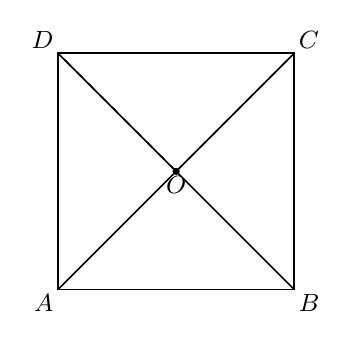
\begin{tikzpicture}[semithick, every node/.style={inner sep=1.4pt, font=\small}]
  \coordinate (A) at (0,0);
  \coordinate (B) at (3,0);
  \coordinate (C) at (3,3);
  \coordinate (D) at (0,3);
  \coordinate (O) at (1.5,1.5);
  \draw (A) -- (B) -- (C) -- (D) -- cycle;
  \draw (A) -- (C);
  \draw (B) -- (D);
  \draw[dashed] (O) -- (C);
  \draw[dashed] (O) -- (D);
  \fill (O) circle (1.3pt);
  \node[below left] at (A) {$A$};
  \node[below right] at (B) {$B$};
  \node[above right] at (C) {$C$};
  \node[above left] at (D) {$D$};
  \node[below] at (O) {$O$};
\end{tikzpicture}
\end{center}
\nopagebreak[4]
\Needspace{0.4\textheight}
\end{question}
\endgroup
\begingroup
\renewenvironment{question}{\Needspace{0.5\textheight}}{}
\begin{question}
\gkti{13}如图，直线 $x=2$ 与双曲线 $\Gamma:\dfrac{x^2}4-y^2=1$ 的渐近线交于 $E_1$、$E_2$ 两点，记 $\overrightarrow{OE_1}=\boldsymbol e_1$，$\overrightarrow{OE_2}=\boldsymbol e_2$，任取双曲线 $\Gamma$ 上的点 $P$，若 $\overrightarrow{OP}=a\boldsymbol e_1+b\boldsymbol e_2$（$a,b\in\mathbf R$），则 $a$、$b$ 满足的一个等式是$\underline{\qquad}$．
\nopagebreak[4]
\begin{center}% 2010 年上海卷理科第 13 题：双曲线 x^2/4-y^2=1 的渐近线与直线 x=2 交于 E1、E2。
% 来源 PDF：普通高考/2010/2010上海理.pdf，SHA-256 e6181a8e02bfda976d5a2cee9432881769c184da4d3fca3b5a4d75c57a497ec6。
% 原页：第 1 页（A3 三栏）第 3 栏中部，书页码 627。
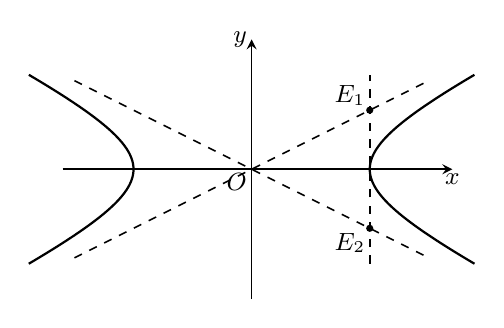
\begin{tikzpicture}[semithick, x=0.75cm, y=0.75cm, every node/.style={inner sep=1.4pt, font=\small}]
  \draw[-stealth] (-3.2,0) -- (3.4,0) node[below] {$x$};
  \draw[-stealth] (0,-2.2) -- (0,2.2) node[left] {$y$};
  \node[below left] at (0,0) {$O$};
  % 双曲线两支
  \draw[domain=-1.6:1.6,samples=80,thick] plot ({2*sqrt(1+\x*\x)},\x);
  \draw[domain=-1.6:1.6,samples=80,thick] plot ({-2*sqrt(1+\x*\x)},\x);
  % 渐近线
  \draw[dashed] (-3,-1.5) -- (3,1.5);
  \draw[dashed] (-3,1.5) -- (3,-1.5);
  % x=2
  \draw[dashed] (2,-1.6) -- (2,1.6);
  \fill (2,1) circle (1.3pt);
  \fill (2,-1) circle (1.3pt);
  \node[above left] at (2,1) {$E_1$};
  \node[below left] at (2,-1) {$E_2$};
\end{tikzpicture}
\end{center}
\nopagebreak[4]
\end{question}
\endgroup
\begin{question}
\gkti{14}从集合 $U=\{a,b,c,d\}$ 的子集中选出 $4$ 个不同的子集，需同时满足以下两个条件：

（1）$\varnothing$，$U$ 都要选出；

（2）对选出的任意两个子集 $A$ 和 $B$，必有 $A\subseteq B$ 或 $A\supseteq B$．

那么，共有$\underline{\qquad}$种不同的选法．

\end{question}
\gkpart{二、选择题}

\begin{question}
\gkti{15}“$x=2k\pi+\dfrac\pi4$（$k\in\mathbf Z$）”是“$\tan x=1$”成立的（　）

（A）充分不必要条件

（B）必要不充分条件

（C）充要条件

（D）既不充分也不必要条件

\end{question}
\begin{question}
\gkti{16}直线 $l$ 的参数方程是 $\begin{cases}x=1+2t,\\ y=2-t,\end{cases}$（$t\in\mathbf R$），则 $l$ 的方向向量 $\boldsymbol d$ 可以是（　）

（A）$(1,2)$

（B）$(2,1)$

（C）$(-2,1)$

（D）$(1,-2)$

\end{question}
\begin{question}
\gkti{17}若 $x_0$ 是方程 $\left(\dfrac12\right)^x=x^{\frac13}$ 的解，则 $x_0$ 属于区间（　）

（A）$\left(\dfrac23,1\right)$

（B）$\left(\dfrac12,\dfrac23\right)$

（C）$\left(\dfrac13,\dfrac12\right)$

（D）$\left(0,\dfrac13\right)$

\end{question}
\begin{question}
\gkti{18}某人要作一个三角形，要求它的三条高的长度分别是 $\dfrac1{13}$、$\dfrac1{11}$、$\dfrac15$，则此人将（　）

（A）不能作出满足要求的三角形

（B）作出一个锐角三角形

（C）作出一个直角三角形

（D）作出一个钝角三角形

\end{question}
\gkpart{三、解答题}

\begin{question}
\gkti{19}已知 $0<x<\dfrac\pi2$，化简：

\nopagebreak[4]
\[\lg\left(\cos x\cdot\tan x+1-2\sin^2\frac x2\right)
+\lg\left[\sqrt2\cos\left(x-\frac\pi4\right)\right]
-\lg(1+\sin2x).\]

\end{question}
\begin{question}
\gkti{20}已知数列 $\{a_n\}$ 的前 $n$ 项和为 $S_n$，且 $S_n=n-5a_n-85$，$n\in\mathbf N^*$．

（1）证明：$\{a_n-1\}$ 是等比数列；

（2）求数列 $\{S_n\}$ 的通项公式，并指出 $n$ 为何值时，$S_n$ 取得最小值，并说明理由．

\Needspace{0.4\textheight}
\end{question}
\begingroup
\renewenvironment{question}{\Needspace{0.5\textheight}}{}
\begin{question}
\gkti{21}如图，为了制作一个圆柱形灯笼，先要制作 $4$ 个全等的矩形骨架，总计耗用 $9.6$ 米铁丝．骨架将圆柱底面 $8$ 等分，再用 $S$ 平方米塑料片制成圆柱的侧面和下底面（不安装上底面）．

（1）当圆柱底面半径 $r$ 取何值时，$S$ 取得最大值？并求出该最大值（结果精确到 $0.01$ 平方米）；

（2）在灯笼内，以矩形骨架的顶点为端点，安装一些霓虹灯．当灯笼底面半径为 $0.3$ 米时，求图中两根直线型霓虹灯 $A_1B_3$、$A_3B_5$ 所在异面直线所成角的大小（结果用反三角函数表示）．
\nopagebreak[4]
\begin{center}% 2010 年上海卷理科第 21 题：圆柱形灯笼、底面 8 等分与霓虹灯 A1B3、A3B5。
% 来源 PDF：普通高考/2010/2010上海理.pdf，SHA-256 e6181a8e02bfda976d5a2cee9432881769c184da4d3fca3b5a4d75c57a497ec6。
% 原页：第 2 页（A3 三栏）第 1 栏上部，书页码 628。
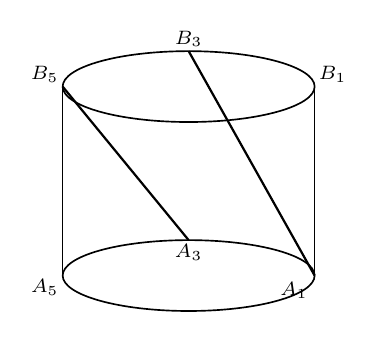
\begin{tikzpicture}[semithick, every node/.style={inner sep=1.2pt, font=\scriptsize}]
  % 下底与上口
  \draw (0,0) ellipse (1.6 and 0.45);
  \draw (0,2.4) ellipse (1.6 and 0.45);
  \draw (-1.6,0) -- (-1.6,2.4);
  \draw (1.6,0) -- (1.6,2.4);
  % 八个分点
  \foreach \a/\n in {0/1,45/2,90/3,135/4,180/5,225/6,270/7,315/8}{
    \coordinate (A\n) at ({1.6*cos(\a)},{0.45*sin(\a)});
    \coordinate (B\n) at ({1.6*cos(\a)},{2.4+0.45*sin(\a)});
  }
  % 霓虹灯
  \draw[thick] (A1) -- (B3);
  \draw[thick] (A3) -- (B5);
  % 标注关键点
  \node[below left=1pt] at (A1) {$A_1$};
  \node[below] at (A3) {$A_3$};
  \node[below left] at (A5) {$A_5$};
  \node[above] at (B3) {$B_3$};
  \node[above left] at (B5) {$B_5$};

  \node[above right] at (B1) {$B_1$};
\end{tikzpicture}
\end{center}
\nopagebreak[4]
\end{question}
\endgroup
\begin{question}
\gkti{22}若实数 $x$、$y$、$m$ 满足 $|x-m|>|y-m|$，则称 $x$ 比 $y$ 远离 $m$．

（1）若 $x^2-1$ 比 $1$ 远离 $0$，求 $x$ 的取值范围；

（2）对任意两个不相等的正数 $a$、$b$，证明：$a^3+b^3$ 比 $a^2b+ab^2$ 远离 $2ab\sqrt{ab}$；

（3）已知函数 $f(x)$ 的定义域 $D=\left\{x\mid x\neq\dfrac{k\pi}2+\dfrac\pi4,\ k\in\mathbf Z,\ x\in\mathbf R\right\}$．任取 $x\in D$，$f(x)$ 等于 $\sin x$ 和 $\cos x$ 中远离 $0$ 的那个值．写出函数 $f(x)$ 的解析式，并指出它的基本性质（结论不要求证明）．

\Needspace{0.4\textheight}
\end{question}
\begingroup
\renewenvironment{question}{\Needspace{0.5\textheight}}{}
\begin{question}
\gkti{23}已知椭圆 $\Gamma$ 的方程为 $\dfrac{x^2}{a^2}+\dfrac{y^2}{b^2}=1$（$a>b>0$），点 $P$ 的坐标为 $(-a,b)$．

（1）若直角坐标平面上的点 $M$、$A(0,-b)$、$B(a,0)$ 满足 $\overrightarrow{PM}=\dfrac12\left(\overrightarrow{PA}+\overrightarrow{PB}\right)$，求点 $M$ 的坐标；

（2）设直线 $l_1:y=k_1x+p$ 交椭圆 $\Gamma$ 于 $C$、$D$ 两点，交直线 $l_2:y=k_2x$ 于点 $E$．若 $k_1\cdot k_2=-\dfrac{b^2}{a^2}$，证明：$E$ 为 $CD$ 的中点；

（3）对于椭圆 $\Gamma$ 上的点 $Q(a\cos\theta,b\sin\theta)$（$0<\theta<\pi$），如果椭圆 $\Gamma$ 上存在不同的两点 $P_1$、$P_2$ 使 $\overrightarrow{PP_1}+\overrightarrow{PP_2}=\overrightarrow{PQ}$，写出求作点 $P_1$、$P_2$ 的步骤，并求出使 $P_1$、$P_2$ 存在的 $\theta$ 满足的条件．
\nopagebreak[4]
\begin{center}% 2010 年上海卷理科第 23 题：椭圆 Γ 与点 P(-a,b)、Q(a cosθ,b sinθ)。
% 来源 PDF：普通高考/2010/2010上海理.pdf，SHA-256 e6181a8e02bfda976d5a2cee9432881769c184da4d3fca3b5a4d75c57a497ec6。
% 原页：第 2 页（A3 三栏）第 3 栏下部，书页码 628。
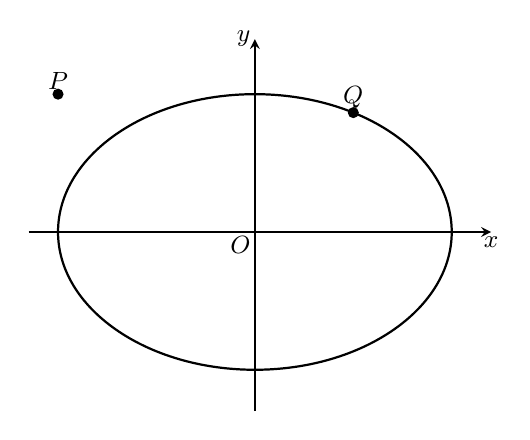
\begin{tikzpicture}[semithick, x=0.25cm, y=0.35cm, every node/.style={inner sep=1.3pt, font=\small}]
  \draw[-stealth] (-11.5,0) -- (12,0) node[below] {$x$};
  \draw[-stealth] (0,-6.5) -- (0,7) node[left] {$y$};
  \node[below left] at (0,0) {$O$};
  \draw[thick] (0,0) ellipse (10 and 5);
  \coordinate (P) at (-10,5);
  \coordinate (Q) at (5,4.330);
  \fill (P) circle (2pt);
  \fill (Q) circle (2pt);
  \node[above] at (P) {$P$};
  \node[above] at (Q) {$Q$};
\end{tikzpicture}
\end{center}
\nopagebreak[4]

\end{question}
\endgroup